\documentclass{article}


\usepackage[a4paper]{geometry}
\usepackage[british]{babel}
\usepackage{amsmath,amssymb,euscript,enumitem}

\def\barroman#1{\sbox0{#1}\dimen0=\dimexpr\wd0+1pt\relax
  \makebox[\dimen0]{\rlap{\vrule width\dimen0 height 0.06ex depth 0.06ex}%
    \rlap{\vrule width\dimen0 height\dimexpr\ht0+0.03ex\relax 
            depth\dimexpr-\ht0+0.09ex\relax}%
    \kern.5pt#1\kern.5pt}}

\usepackage{tikz}
\usetikzlibrary{patterns}
\usetikzlibrary{shapes.geometric, calc}
%\usetikzlibrary{positioning}

\usepackage{hyperref}
\usepackage{color}
\definecolor{darkgreen}{RGB}{0,100,0}
\definecolor{firebrick}{RGB}{178,34,34}

\newenvironment{proof}[1][{}]{%\novbskip%
  \begin{trivlist}\item[]\textit{Proof #1}\quad}%
  {\hfill\hspace*{\fill}~$\square$\end{trivlist}}

\newtheorem{theorem}{Theorem}[section]
\newtheorem{proposition}[theorem]{Proposition}
\newtheorem{claim}[theorem]{Claim}
\newtheorem{conjecture}[theorem]{Conjecture}
\newtheorem{lemma}[theorem]{Lemma}
\newtheorem{definition}[theorem]{Definition}
\newtheorem{corollary}[theorem]{Corollary}
\newtheorem{example}[theorem]{Example}
\newtheorem{remark}[theorem]{Remark}

\DeclareMathOperator{\bdr}{bdr}
\DeclareMathOperator*{\argmin}{argmin}

\newcommand{\ud}{\mathrm{d}}
\newcommand\R{\mathbb{R}}
\newcommand{\grad}{\mathrm{grad}}
\newcommand{\M}{\mathcal{M}}
\newcommand{\Su}{\mathcal{S}}
\newcommand{\rch}{\mathrm{rch}}
\newcommand\abs[1]{\left\lvert#1\right\rvert}
\newcommand\norm[1]{\left\lVert #1 \right\rVert}
\newcommand{\diff}{\mathop{}\mathopen{}\mathrm{d}}
\newcommand{\intervalle}[4]{\mathopen{#1}#2\mathpunct{};#3\mathclose{#4}}
\newcommand{\intervalleff}[2]{\intervalle{[}{#1}{#2}{]}}
\newcommand{\intervalleof}[2]{\intervalle{]}{#1}{#2}{]}}
\newcommand{\intervallefo}[2]{\intervalle{[}{#1}{#2}{[}}
\newcommand{\intervalleoo}[2]{\intervalle{]}{#1}{#2}{[}}
\newcommand{\bulletitem}{\item[\textbullet]}
\newcommand\ie{\emph{i.e.}\ }


\newcommand{\phant}{{\vphantom{-1}}} % used to have invisible superscripts so the subscripts are on the same heigh

% taille du papier et marges
\geometry{papersize={21cm,29.7cm}}
\geometry{hmargin=2cm, bottom=5cm, top=2cm}

\begin{document}
\title{convexity}
\author{}
\maketitle

\section{Introduction}





\subsection{Definitions and notation} 

We assume that $\M$ is a closed $n$-dimensional smooth manifold without boundary, embedded in $\mathbb{R}^d$. The tangent bundle is denoted by $T\M$ and the tangent plane at the point $p \in \M$ by $T_p \M$, which we shall often regard as embedded in $\mathbb{R}^d$ without explicitly refering to the embedding. The normal bundle will be denoted by $N\M$ and the normal space at a point $p\in \M$ by $N_p\M$. We will write $N_p^{\mathbb{E}}\M=( T_p \M )^{\perp} $ for the canonical embedding of $N_p\M$ in $\mathbb{R}^d$ as the affine space orthogonal to $T_p\M$.


Geodesic distances on manifolds between $x,y \in \M$ are denoted by $d_\M(x,y)$. The distance between the points $x$ and $y$ in Euclidean space is denoted by $|x-y|$, while the Euclidean distance between a point $x$ and a subset $A$ is 
\begin{align} 
d_{\mathbb{E}} (x,A) = \min_{y \in A}  |x-y| .  
\nonumber 
\end{align}
Inner products are denoted by $\langle \cdot , \cdot \rangle$. 
A straight line segment in $\mathbb{R}^d$ is denoted by $[ab]$. Angles between two line segments $[ab]$, $[cd]$ or a line segment $[bc]$ and an affine subspace $A$ will be denoted by $\angle ([ab], [cd] )$ or $\angle ([bc], A)  $ respectively.

For an embedded manifold, the medial axis ($\textrm{ax}(\M)$) is the set of points in the ambient space for which there are at least two points on the manifold that attain the minimal distance to the point in ambient space. The reach of $\M$ is the minimal distance from the medial axis to the manifold and is denoted by $\rch(\M)$.

Projections are generally denoted by $\pi$. The orthogonal projection of points in $\mathbb{R}^d$ onto the tangent plane $T_p \M$ as $\pi_{T_p \M}: \mathbb{R}^d \to  T_p \M$.  Let $N(\M, r)= \{x \in \mathbb{R}^d \mid d_{\mathbb{E}} (x, \M) <r\} $ be a neighbourhood of radius $r < \rch (\M)$. The projection of a point $x \in N(\M, r)$, again with $r< \rch (\M)$, onto the closest point on $\M$ will be denoted by $\pi_\M$.


\section{Tubular neighbourhoods and empty balls} 
We shall be using the following result, Theorem 4.8(12) of \cite{federer1959}:
\begin{theorem}[Federer's tubular neighbourhoods for $C^{1,1}$ manifolds] \label{Theorem:TubularNeighbourhood}
Let $B_{N_p\M} (r)$, be the ball of radius $r$ centred at $p$ in the normal space $N_p^{\mathbb{E}}\M\subset \mathbb{R}^d$ of a $C^{1,1}$ manifold $\M$ with reach $\rch ( \M)$, where $r< \rch (\M)$. For every point $x \in B_{N_p\M} (r)$, again with $r< \rch (\M)$, $\pi_{\M}(x)=p$.
\end{theorem}

From Theorem \ref{Theorem:TubularNeighbourhood} we immediately see that: 
\begin{corollary}
\label{lem:medialball}
Let $\M$ be a submanifold of $\mathbb{R}^d$ and $p\in \M$. Any open ball $B(c,r)$ that is tangent to $\M$ at $p$ and whose radius $r$ satisfies $r\leq \rch (\M)$ does not intersect $\M$.
\end{corollary}
\begin{proof} Let $r < \rch (\M)$.
Suppose that the intersection of $\M$ and the open ball is not empty, then the $\pi_{\M}(c)\neq p$ contradicting Federer's tubular neighbourhood theorem. The result for $r=  \rch (\M)$ now follows by taking the limit.
\end{proof}

For a full discussion, including a historical overview, we refer to {\color{red} cite full version of the other paper}. 

%On note $V_x$ un voisinage de $x$ tel que la boule de centre $c$ et de rayon $|x-c|$ n'intersecte pas $K \cap V_x$ (ce voisinage existe par définition de boule tangente). On considère ensuite la fonction suivante (avec vos notations):
%\[f(\lambda) := d_{K'}(c(\lambda)) - \|c(\lambda) - x\|,\]
%ou $K' = K \cap (R^d \setminus V_x)$ est la restriction de $K$ au complémentaire de $V_x$.














\section{Convexity}


We start with a very simple observation concerning the reach of a manifold:
\begin{lemma}
\label{lem:ReachSecondDer}
Let $\gamma(t)$ be a geodesic parametrized according to arc length on $\M \subset \mathbb{R}^d$, then $|\ddot{\gamma} | \leq 1/ \rch (\M)$, where we use Newton's notation, that is we write $\ddot{\gamma}$ for the second derivative of $\gamma$ with respect to $t$. 
\end{lemma}
\begin{proof} 
Because $\gamma(t)$ is a geodesic, $\ddot{\gamma}(t)$ is normal to $\M$ at $\gamma(t)$. Now consider the sphere of radius $\rch(\M)$ tangent to $\M$ at $\gamma(t)$, whose centre lies on the line $\{ \gamma(t)+ \lambda \ddot{\gamma}  \mid \lambda \in \mathbb{R} \}$. If now $|\ddot{\gamma} | $ were larger than $1/ \rch (\M)$, the geodesic $\gamma$ would enter the tangent sphere, which would contradict Corollary \ref{lem:medialball}.
\end{proof}

Note that $|\ddot{\gamma} | $ is the normal curvature, because $\gamma$ is a geodesic. Using the terminology of \cite[Section 6]{niyogi2008}, Lemma \ref{lem:ReachSecondDer} can also be formulated as follows: $1/ \rch (\M)$ bounds the principal curvatures in the normal direction $\nu$, for any unit normal vector $\nu\in N_p \M$. In particular, $1/ \rch (\M)$ also bounds the pricipal curvatures in the codimension one setting. 


We now have the following, as we have seen in \cite{attali:hal-00201055} for surfaces and in \cite{TangentVar}: 

Assume that $p,q \in \M $, such that $d_\M (p,q) \leq \pi \rch(\M)$. 
Let $\gamma$ be a geodesic parametrized according to arc length whose length $\ell$ therefore equals $d_\M (p,q)$, such that $\gamma(0)=p$ and $\gamma(\ell)=q$. Because $\gamma$ is parametrized according to arc length $| \dot{\gamma} |=1$ and $\dot{\gamma}(t)$ can be seen as a curve on the sphere $\mathbb{S}^{d-1}$. Moreover $\ddot{\gamma}$ can be seen as tangent to this sphere. The angle between two tangent vectors $\dot{\gamma}(a)$ and $\dot{\gamma}(b)$ equals the geodesic distance on the sphere. The geodesic distance between any two points is smaller or equal to the length of any curve connecting these points, and $\{\dot{\gamma}(t) \mid t \in [a,b] \}$ is such a curve. We therefore have
\begin{align}
\angle \dot{\gamma}(a) \dot{\gamma}(b) 
\leq \int_{a}^{b} \left | \frac{d}{dt} \dot{\gamma} \right| \ud t 
=\int_{a}^{b} |  \ddot{\gamma} | \ud t 
\leq \frac{|a-b| } {\rch(\M)} ,
\label{eq:angleEst1}
\end{align}
where we used Lemma \ref{lem:ReachSecondDer}. 

This result was used (in \cite{attali:hal-00201055,TangentVar}) to prove the following lemma 
\begin{lemma}
\label{lem:TightMetricDist} 
Let $p,q \in \M $ be such that $d_\M (p,q) \leq \pi \rch(\M)$, then
\begin{align}
2 \, \rch(\M) \sin \left(\frac{ d_\M (p,q)}{2\rch(\M)} \right)\leq |p-q|.
\nonumber
\end{align}
\end{lemma} 

Here we shall use the estimate \eqref{eq:angleEst1} to prove the following:
\begin{lemma}
\label{Lem:Orthogonal_distance} 
Let $p,q \in \M $ be such that $d_\M (p,q) <\pi \rch(\M)$ and let $\gamma(t)$ be a minimizing geodesic parametrized by arc length connecting $p$ and $q$, then
\begin{align}
d_\mathbb{E}(\gamma(t) , [pq]) =\ell \leq \rch(\M)
 \left (\cos \frac{|\ell /2-t| } {\rch(\M)}  -\cos \frac{\ell} {2 \rch(\M)}\right ).
\nonumber
\end{align}
\end{lemma} 
\begin{proof} 
We shall denote the orthogonal projection onto $[pq]$ by $\pi_{[pq]}$ and the direction of the line segment $[pq]$ by $z$. We now consider the two dimensional curve $\tilde{\gamma}(t)= (\tilde{\gamma}_z(t),\tilde{\gamma}_\rho(t))= (\pi_{[pq]}(\gamma(t)), |\gamma(t)-\pi_{[pq]}(\gamma(t) )| ) $. The geometric interpretation is the following: We first consider $\gamma(t)$ in cylindrical coordinates, where we regard the line that extends $[pq]$ as the `$z$-axis'. We then project on the radial $\rho$ and `$z$'-direction. We also refer to the unit vector in the radial direction as $\rho$. 

\begin{figure}[h!]
\centering
\includegraphics[width=.9\textwidth]{pictures/QsiddharthJDCurve}
\caption{A sketch of the curves $\gamma(t)$ (blue), $\tilde{\gamma}(t)$ (green), and the line segment $[pq]$ (red). The $\rho,z$-plane is indicated in greyish green.}
\label{SketchGamma}
\end{figure}

Observe that $\dot{\tilde{\gamma}}(t)$ is the projection on the $\rho,z$-plane of $\dot{\gamma}(t)$ and thus
\begin{align} 
\angle \dot{\tilde{\gamma}}(a) \dot{\tilde{\gamma}}(b) \leq \angle \dot{\gamma}(a) \dot{\gamma}(b),
\nonumber
\end{align} 
because any projection decreases angles. Using \eqref{eq:angleEst1} we now see that 
\begin{align} 
\angle \dot{\tilde{\gamma}}(a) \dot{\tilde{\gamma}}(b) \leq \frac{|a-b| } {\rch(\M)}.
\label{eq:angleEst2}
\end{align}
We also note that $|\dot{\tilde{\gamma}}(t)|\leq 1$.

Let $s^*\in [0 , \ell]$ be a point such that $ \frac{d}{dt} (\tilde{\gamma}_\rho(t)) \mid_{t=s^*} = 0$, that is $\dot{\tilde{\gamma}}(s^*)$ lies in the $z$-direction. 
There exists such an $s^*$ for there is a point where the maximum of $\tilde{\gamma}_\rho(t)$ is attained. By possibly interchanging the roles of $p$ and $q$ we can assume that $s^*\leq \ell/2$. 

We now have the following estimate
\begin{align}
d_{\mathbb{E}}(\gamma(s^*) , [pq]) & \leq  \left| \int_{0}^{s^*} \langle  \rho, \dot{\tilde{\gamma}}(s) \rangle \ud s \right| 
\nonumber
\\ 
&
\leq  \int_{0}^{s^*} |\langle  \rho, \dot{\tilde{\gamma}}(s) \rangle | \ud s  
\nonumber
\\
&
\leq \int_{0}^{s^*} \cos \angle \rho \dot{\tilde{\gamma}}(s) \ud s
\nonumber
\\
&
= \int_{0}^{s^*} \sin \angle z \dot{\tilde{\gamma}}(s) \ud s
\nonumber
\\
&
= \int_{0}^{s^*} \sin \angle \dot{\tilde{\gamma}}(s^*) \dot{\tilde{\gamma}}(s) \ud s
\nonumber
\\
&
\leq \int_{0}^{s^*} \sin \frac{|s-s^*| } {\rch(\M)}  \ud s
\nonumber
\\
& 
= \rch(\M)
 \left (1-\cos \frac{s^* } {\rch(\M)}  \right ),
\nonumber
\end{align}
where the third inequality is due to the fact that $|\dot{\gamma }|\leq 1$ and the last inequality is due to \eqref{eq:angleEst2}. It is clear that the bound is maximized if $s^*=\ell/2$. This maximum is attained for the sphere of the appropriate dimension. 

We can now do the same analysis for any $t \in [0 ,s^*]$. We see that 
\begin{align}
d_{\mathbb{E}}(\gamma(t)  , [pq]) & \leq  \left| \int_{0}^{t } \langle  \rho, \dot{\tilde{\gamma}}(s) \rangle \ud s \right| 
\nonumber
\\
&
\leq \int_{0}^{t} \sin \angle \dot{\tilde{\gamma}}(s^*) \dot{\tilde{\gamma}}(s) \ud s
\nonumber
\\
&
\leq \int_{0}^{t} \sin \frac{|s-s^*| } {\rch(\M)}  \ud s
\nonumber
\\
& 
\leq \rch(\M)
 \left ( \cos \frac{|s^*-t| } {\rch(\M)} -\cos \frac{s^* } {\rch(\M)} \right ),
\nonumber
\end{align}
which again is maximized if $s^*=\ell/2$ and attained for the sphere.
\end{proof}

We also need the following lemma:
\begin{lemma}
\label{lem:ConditionAmbientSpace} 
Let $\M$ be a compact $C^2$ manifold and $p,q \in \M $ be such that $|p-q| < 2 \rch(\M)$, then $d_\M (p,q) < \pi \rch(\M)$.
\end{lemma}
\begin{proof}
We first note that if $|p-q| < 2 \rch (\M)$, then $p$ and $q$ lie on the same connected component of $\M$. If fact we shall prove that if $p$ and $q$ lie on different connected components then $|p-q| \geq 2 \rch(\M)$. Let $\M_1$ and $\M_2$ be two connected components of $\M$ with the smallest distance between them, if there is more than one such pair we pick one. We may assume that $p$ lies on $\M_1$ and $q$ on $\M_2$. Consider points the $x \in \M_1$ and $y \in  \M_2$, where the distance $d(\M_1,\M_2)$ is attained. The line segment $[xy]$ is normal to both $\M_1$ and $\M_2$, from which we can conclude that the midpoint of $[xy]$ is equidistant to both $\M_1$ and $\M_2$. Moreover there cannot be another connected component of $\M$ that is closer to the midpoint because we assumed that $\M_1$ and $\M_2$ are the two connected components that are the closest. This means that the midpoint lies on the medial axis. Our claim now follows. We can now safely assume that $\M$ has one connected component.

Thanks to Lemma \ref{lem:TightMetricDist}, we know that the if $d_\M(p,q) = \pi \rch(\M)$, then $|p-q|\geq 2 \rch(\M)$. This means that we can subdivide $\M$ in $B_{\M}(p,\pi \rch(\M))$, the geodesic ball of radius $\pi \rch(\M)$, and $\M \setminus B_{\M}(p,\pi \rch(\M))$. Now suppose that $(\M \setminus B_{\M}(p,\pi \rch(\M))) \cap B(p, 2 \rch(\M)) \neq \emptyset$, with $B(p, 2 \rch(\M))$ the open Euclidean ball of radius $2 \rch(\M)$. We pick the point $y \in (\M \setminus B_{\M}(p,\pi \rch(\M))) \cap B(p, 2 \rch(\M)$ that is the closest to $p$. We now see that
\begin{itemize}
\item $[yp]$ is normal to $\M$ at $y$ and thus for all $x \in [yp]$ with $|x-y| < \rch(\M)$, $\pi_\M (x)= y$, by Federer's tubular neighbourhood theorem.
\item $|y-p| < 2 \rch (\M)$
\end{itemize} 
For any $0 <\epsilon < \rch(\M) -|y-p|/2$, we can pick the point $x \in [yp]$ with is a distance $\rch(\M)-\epsilon$ from $y$. Due to Federer's tubular neighbourhood theorem $\pi_\M (x) =y$ but by construction $x$ closer to $p$, a contradiction. 
\end{proof}


Lemmas \ref{Lem:Orthogonal_distance} and \ref{lem:ConditionAmbientSpace} tell us that the geodesic connecting $p$ and $q$ is contained in the lens shaped region $L_{pq}$, where $L_{pq}$ is constructed as follows. We first take the circle of radius equal to the reach $\rch (\M)$, such that the line $[pq]$ is a chord. This chord divides the circle in two parts. $L_{pq}$ is the hypersurface of revolution found by revolving the shortest part of the circle, denoted by $C_{s,[pq]}$, around $[pq]$. 

\begin{figure}[!h]
    \centerline{
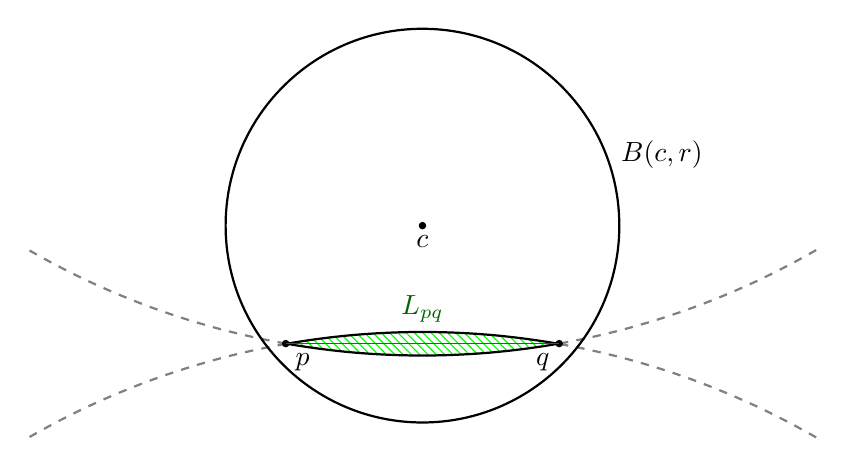
\begin{tikzpicture}
\coordinate [label={below right:$p$}] (p) at ({10*cos(260)}, {10*sin(260)+9.85});
\coordinate [label={below left:$q$}] (q) at ({10*cos(280)}, {10*sin(280)+9.85});
\fill [pattern=north west lines, pattern color=green, domain=260:280, variable=\x]
  plot ({10*cos(\x)}, {10*sin(\x)+9.85})
  -- cycle;
\fill [pattern=north west lines, pattern color=green, domain=80:100, variable=\x]
  plot ({10*cos(\x)}, {10*sin(\x)-9.85})
  -- cycle;
\draw [thick,domain=80:100] plot ({10*cos(\x)}, {10*sin(\x)-9.85});
\draw [thick,domain=260:280] plot ({10*cos(\x)}, {10*sin(\x)+9.85});
\draw [gray, thick, dashed, domain=60:80] plot ({10*cos(\x)}, {10*sin(\x)-9.85});
\draw [gray, thick, dashed, domain=260:240] plot ({10*cos(\x)}, {10*sin(\x)+9.85});
\draw [gray, thick, dashed ,domain=100:120] plot ({10*cos(\x)}, {10*sin(\x)-9.85});
\draw [gray, thick, dashed ,domain=300:280] plot ({10*cos(\x)}, {10*sin(\x)+9.85});
\draw[fill] (q) circle (0.04);
\draw[fill] (p) circle (0.04);
\coordinate [label={below:$c$}] (c) at (0,1.5);
\draw [thick, black] (c) circle [radius=2.5];
\draw[fill] (c) circle (0.04);
\draw [red] (p)--(q);
\coordinate [label={above:{\color{darkgreen}$L_{pq}$}}] (L) at (0,0.15);
\coordinate [label={right:$B(c,r)$}] (c) at (2.4,2.4);
\end{tikzpicture}
    }
\caption{The lens shaped region $L_{pq}$ is indicated in green, the grey dashed circles have radius $\rch(\M)$. We see that $L_{pq}\subset B(c,r)$. } 
\label{fig:lens}
\end{figure}


Let $B(c,r)$ be a sphere of radius $r < \rch(\M)$ and let $p$ and $q$ now be any points in $B(c,r)$. Eventually we shall again impose that $p$ and $q$ lie on $\M$, but we ignore this for the moment. We claim that $L_{pq}$ is completely contained in $B(c,r)$. 
%Suppose it is not contained, and $L_{pq}$ intersects $B(c,r)$ in a point $x$. 
Consider any affine plane $P$ spanned by containing $[pq]$. We look at the two circles of radius $\rch(\M)$ in this plane, such $[pq]$ is a chord. Because these circles of radius $\rch(\M)$ have larger radius than the circle $B(c,r)\cap P$, the shortest parts of the circles of radius $\rch(\M)$, namely $C_{s,[pq]}$ and its mirror image, lie inside $B(c,r)\cap P$. 

We are now ready to prove the following theorem:
\begin{theorem}
Let $\M$ be a compact $C^2$ manifold embedded in $\mathbb{R}^d$ and $B(c,r)$ a ball of radius $r<\rch(\M)$. Then $\M \cap B(c,r)$ is geodesically convex, in the sense that the minimizing geodesic connecting any two points in $\M \cap B(c,r)$ is itself contained in $\M \cap B(c,r)$. 
\end{theorem}
\begin{proof}
For any two points $p,q \in \M \cap B(c,r)$, we consider the geodesic $\gamma(t)$ connecting $p$ and $q$. As we have seen above $\gamma \subset L_{pq}$ and trivially $\gamma \subset \M$, so 
\begin{align}
\gamma \subset  L_{pq} \cap \M \subset B(c,r) \cap \M.
\nonumber
\end{align} 
\end{proof}

It trivially follows that $\M \cap B(c,r)$ is a topological ball. 

\section*{Acknowledgements} 
We thank Ramsay Dyer for discussion. The research leading to these results has received funding from the European Research Council (ERC) under  the  European  Union's  Seventh  Framework  Programme (FP/2007-2013)  /  ERC  Grant Agreement No. 339025 GUDHI (Algorithmic Foundations of Geometry Understanding in Higher Dimensions).
\phantomsection
\bibliographystyle{alpha}
\addcontentsline{toc}{section}{Bibliography}
%\bibliographystyle{plain}
\bibliography{ref}





\end{document}
